% !TeX program = xelatex
\documentclass[a4paper,10pt]{article}

% ============================================================================
% កញ្ចប់បណ្ណាល័យ (Packages) – អនុវិទ្យាល័យព្រះក្រសាំង (គ្មាន LCD / សន្លឹកកិច្ចការជាគោល)
% ============================================================================
\usepackage[a4paper, left=0.95cm, right=0.95cm, top=0.85cm, bottom=0.92cm, footskip=0.52cm]{geometry}
\usepackage{amsmath}
\usepackage{unicode-math}
\usepackage{fontspec}
\usepackage{array, longtable, multirow, colortbl}
\usepackage[table]{xcolor}
\usepackage{enumitem}
\usepackage{pifont}
\usepackage{fancyhdr}
\usepackage{tikz}
\usetikzlibrary{calc, arrows.meta, decorations.pathreplacing, patterns, positioning, babel}

% LaTeX + longtable compatibility guard
\makeatletter
\let\@expl@@@mark@update@singlecol@structures@@\relax
\makeatother

% ============================================================================
% ការកំណត់ពុម្ពអក្សរ (Cross-Platform Windows + Linux Cloud fonts/)
% ============================================================================
\providecommand{\NGSFindFonts}{%
  \IfFileExists{C:/Windows/Fonts/cambria.ttc}{%
    \def\NGSSysPath{C:/Windows/Fonts/}%
    \def\NGSUserPath{C:/Users/KIT/AppData/Local/Microsoft/Windows/Fonts/}%
  }{%
    \IfFileExists{./fonts/KhmerOSsiemreap.ttf}{\def\NGSSysPath{./fonts/}\def\NGSUserPath{./fonts/}}{%
    \IfFileExists{../fonts/KhmerOSsiemreap.ttf}{\def\NGSSysPath{../fonts/}\def\NGSUserPath{../fonts/}}{%
    \IfFileExists{../../fonts/KhmerOSsiemreap.ttf}{\def\NGSSysPath{../../fonts/}\def\NGSUserPath{../../fonts/}}{%
    \IfFileExists{../../../fonts/KhmerOSsiemreap.ttf}{\def\NGSSysPath{../../../fonts/}\def\NGSUserPath{../../../fonts/}}{%
    \IfFileExists{../../../../fonts/KhmerOSsiemreap.ttf}{\def\NGSSysPath{../../../../fonts/}\def\NGSUserPath{../../../../fonts/}}{%
    \IfFileExists{../../../../../fonts/KhmerOSsiemreap.ttf}{\def\NGSSysPath{../../../../../fonts/}\def\NGSUserPath{../../../../../fonts/}}{%
    \IfFileExists{../../../../../../fonts/KhmerOSsiemreap.ttf}{\def\NGSSysPath{../../../../../../fonts/}\def\NGSUserPath{../../../../../../fonts/}}{%
      \def\NGSSysPath{../../../../../../../fonts/}\def\NGSUserPath{../../../../../../../fonts/}%
    }}}}}}}%
  }%
}
\NGSFindFonts

\setmathfont[
  Path={\NGSSysPath},
  FontIndex=1,
  Scale=1.02
]{cambria.ttc}

\defaultfontfeatures{Ligatures=TeX}

\setmainfont[
  Path={\NGSUserPath},
  Extension=.ttf,
  Script=Khmer,
  BoldFont={KhmerOSsiemreap},
  BoldFeatures={FakeBold=1.8},
  ItalicFont={KhmerOSsiemreap},
  ItalicFeatures={FakeSlant=0.25},
  BoldItalicFont={KhmerOSsiemreap},
  BoldItalicFeatures={FakeBold=1.8, FakeSlant=0.25}
]{KhmerOSsiemreap}

\newfontfamily\muol[
  Path={\NGSUserPath},
  Extension=.ttf,
  Script=Khmer
]{KhmerOSmuollight}

\newfontfamily\TimesEn[
  Path={\NGSSysPath},
  Extension=.ttf,
  Scale=1.00,
  BoldFont={timesbd},
  ItalicFont={timesi},
  BoldItalicFont={timesbi}
]{times}

\newfontfamily\NagaBold[
  Path={\NGSUserPath},
  Extension=.ttf
]{AKbalthom Naga Bold}

\newfontfamily\CalibriFont[
  Path={\NGSSysPath},
  Extension=.ttf
]{calibri}

\newfontfamily\Tacteing[
  Path={\NGSUserPath}
]{TACTENG.TTF}

\newfontfamily\CourierBullet[
  Path={\NGSSysPath},
  Extension=.ttf
]{cour}
\newcommand{\wcirc}{{\CourierBullet\fontsize{9.5pt}{11pt}\selectfont o}}

\XeTeXlinebreaklocale "km"
\XeTeXlinebreakskip = 0pt plus 1pt minus 0.1pt

% ============================================================================
% ការកំណត់ពណ៌ និងទម្រង់ទំព័រ (Colors & Page Style)
% ============================================================================
\definecolor{stepgray}{HTML}{D9D9D9}
\definecolor{headgray}{HTML}{F2F2F2}
\definecolor{boxgray}{HTML}{D9D9D9}
\definecolor{darkred}{HTML}{C00000}
\definecolor{red5e}{HTML}{FF0000}

\pagestyle{fancy}
\fancyhf{}
\renewcommand{\headrulewidth}{0pt}
\fancyfoot[R]{\CalibriFont\fontsize{11pt}{13pt}\selectfont\thepage}

\setlength{\parindent}{0pt}
\setlength{\parskip}{0pt}
\setlength{\tabcolsep}{3.8pt}

\newcolumntype{L}[1]{>{\raggedright\arraybackslash}p{#1}}

% ============================================================================
% ម៉ាក្រូជំនួយ (Helper Macros)
% ============================================================================
\newcommand{\en}[1]{{\TimesEn #1}}
\newcommand{\enbf}[1]{{\TimesEn\textbf{#1}}}
\newcommand{\unit}[1]{\,\text{\en{#1}}}
\newcommand{\riel}{\,\text{៛}}
\newcommand{\fiveE}[1]{{\NagaBold\fontsize{9.5pt}{13pt}\selectfont\textcolor{red5e}{#1}}}
\newcommand{\timenote}[1]{\textcolor{darkred}{\textit{#1}}}
\newcommand{\redsub}[1]{\textcolor{darkred}{#1}}
\newcommand{\graybox}[1]{\colorbox{boxgray}{\strut\hspace{2pt}#1\hspace{2pt}}}
\newcommand{\ditem}{\tikz[baseline=-0.5ex]\fill (0,0.42ex) -- (0.42ex,0) -- (0,-0.42ex) -- (-0.42ex,0) -- cycle;\hspace{0.3em}}
\newcommand{\cnum}[1]{{\fontsize{10.5pt}{12pt}\selectfont\ding{\numexpr181+#1\relax}}\hspace{0.15em}}
\newcommand{\cfig}[1]{\par\vspace{3pt}{\centering #1\par}\vspace{3pt}}
\newcommand{\stepheader}[1]{\multicolumn{3}{|c|}{\cellcolor{stepgray}\muol #1} \\* \noalign{\hrule height 0.4pt}}
\newcommand{\fboxb}[1]{\begingroup\setlength{\fboxsep}{1.5pt}\fbox{#1}\endgroup}
\newcommand{\khmflourish}{{\Tacteing\fontsize{36pt}{14pt}\selectfont\raisebox{-5pt}{3}}}

% ============================================================================
% ម៉ាក្រូគូសរូប TikZ ស-ខ្មៅ ១០០% (Monochrome B&W TikZ Figures, Black Text, 7.3-7.45 cm)
% ============================================================================

% ១. E1 Engage: ករណីប្រៀបធៀប ទិញសៀវភៅសរសេរ vs អាយុបងប្អូន (លើសន្លឹកកិច្ចការផ្នែក E1)
\newcommand{\figEngagePROPThreeOneOne}{%
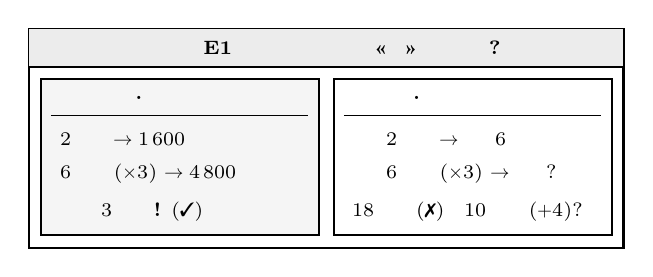
\begin{tikzpicture}[x=1cm, y=1cm, every node/.style={font=\scriptsize, text=black}]
  \draw[black, line width=0.9pt] (0,0) rectangle (7.55,2.78);
  \fill[gray!15] (0,2.30) rectangle (7.55,2.78);
  \draw[black, line width=0.6pt] (0,2.30) -- (7.55,2.30);
  \node at (3.775,2.54) {\textbf{បេសកកម្ម \en{E1}៖ ស្ថានភាពទាំងពីរសុទ្ធតែ «កើន» ដូចគ្នា ឬទេ?}};

  % ប្រអប់ឆ្វេង៖ ហាងលក់សៀវភៅសរសេរ
  \draw[black, line width=0.75pt, fill=gray!8] (0.15,0.16) rectangle (3.68,2.14);
  \node at (1.915,1.90) {\textbf{ក. ថ្លៃសៀវភៅសរសេរ}};
  \draw[black, line width=0.5pt] (0.28,1.68) -- (3.55,1.68);
  \node[anchor=west] at (0.28,1.38) {$2$ ក្បាល $\to 1\,600\riel$};
  \node[anchor=west] at (0.28,0.94) {$6$ ក្បាល ($\times 3$) $\to 4\,800\riel$};
  \node[anchor=west] at (0.28,0.46) {\textbf{គុណនឹង $3$៖ ត្រូវ!} (\ding{51})};

  % ប្រអប់ស្ដាំ៖ អាយុប្អូនដារ៉ា និងបងសុខា
  \draw[black, line width=0.75pt] (3.87,0.16) rectangle (7.40,2.14);
  \node at (5.635,1.90) {\textbf{ខ. អាយុដារ៉ា និងបងសុខា}};
  \draw[black, line width=0.5pt] (4.00,1.68) -- (7.27,1.68);
  \node[anchor=west] at (3.98,1.38) {ដារ៉ា $2$ ឆ្នាំ $\to$ សុខា $6$ ឆ្នាំ};
  \node[anchor=west] at (3.98,0.94) {ដារ៉ា $6$ ឆ្នាំ ($\times 3$) $\to$ សុខា $?$};
  \node[anchor=west] at (3.98,0.46) {$18$ ឆ្នាំ (\ding{55}) ឬ $10$ ឆ្នាំ ($+4$)?};
\end{tikzpicture}}

% ២. E2 Act 1: តារាងផលធៀបជញ្ជីងរ៉ឺស័រ (ទំ.២៧) + ព្រួញពង្រីក និងមេគុណ 0.2
\newcommand{\figExploreSpringPROPThreeOneOne}{%
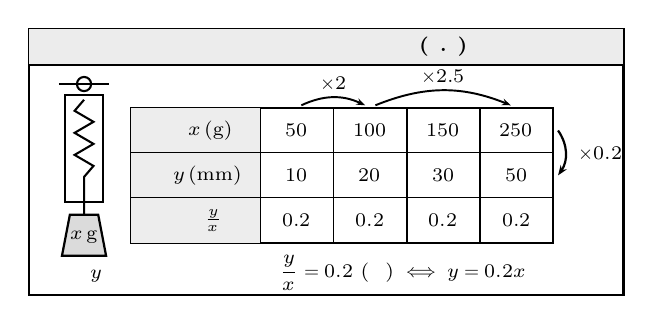
\begin{tikzpicture}[x=1cm, y=1cm, every node/.style={font=\scriptsize, text=black}]
  \draw[black, line width=0.9pt] (0,0) rectangle (7.55,3.38);
  \fill[gray!15] (0,2.92) rectangle (7.55,3.38);
  \draw[black, line width=0.6pt] (0,2.92) -- (7.55,2.92);
  \node at (3.775,3.15) {\textbf{សកម្មភាព ១៖ ជញ្ជីងដៃរ៉ឺស័រ និងតារាងផលធៀប (ទំ.២៧)}};

  % គំនូសតាងជញ្ជីងរ៉ឺស័រខាងឆ្វេង
  \draw[black, line width=0.95pt] (0.38,2.68) -- (1.02,2.68);
  \draw[black, line width=0.75pt] (0.70,2.68) circle (0.09);
  \draw[black, line width=0.8pt] (0.46,1.18) rectangle (0.94,2.54);
  \draw[black, line width=0.75pt] (0.70,2.48) -- (0.58,2.34) -- (0.82,2.20) -- (0.58,2.06) -- (0.82,1.92) -- (0.58,1.78) -- (0.82,1.64) -- (0.70,1.50) -- (0.70,1.02);
  \fill[gray!28, draw=black, line width=0.8pt] (0.42,0.50) -- (0.98,0.50) -- (0.88,1.02) -- (0.52,1.02) -- cycle;
  \node at (0.70,0.74) {$x\unit{g}$};
  \node at (0.70,0.24) {លូត $y$};

  % តារាងផលធៀបខាងស្ដាំ
  \draw[black, line width=0.75pt] (1.30,0.66) rectangle (6.66,2.38);
  \fill[gray!14] (1.30,0.66) rectangle (2.94,2.38);
  \draw[black, line width=0.6pt] (1.30,1.81) -- (6.66,1.81);
  \draw[black, line width=0.6pt] (1.30,1.24) -- (6.66,1.24);
  \foreach \xx in {2.94,3.87,4.80,5.73} {
    \draw[black, line width=0.55pt] (\xx,0.66) -- (\xx,2.38);
  }
  \node at (2.12,2.09) {ម៉ាស $x\unit{(g)}$};
  \node at (2.12,1.52) {លូត $y\unit{(mm)}$};
  \node at (2.12,0.95) {ផលធៀប $\frac{y}{x}$};

  \node at (3.40,2.09) {$50$};   \node at (4.33,2.09) {$100$};
  \node at (5.26,2.09) {$150$};  \node at (6.19,2.09) {$250$};

  \node at (3.40,1.52) {$10$};   \node at (4.33,1.52) {$20$};
  \node at (5.26,1.52) {$30$};   \node at (6.19,1.52) {$50$};

  \node at (3.40,0.95) {$0.2$};  \node at (4.33,0.95) {$0.2$};
  \node at (5.26,0.95) {$0.2$};  \node at (6.19,0.95) {$0.2$};

  \draw[black, line width=0.7pt, -{Stealth[length=3.2pt]}] (3.46,2.41) to[bend left=25] node[above=-1pt]{$\times 2$} (4.27,2.41);
  \draw[black, line width=0.7pt, -{Stealth[length=3.2pt]}] (4.40,2.41) to[bend left=22] node[above=-1pt]{$\times 2.5$} (6.12,2.41);
  \draw[black, line width=0.8pt, -{Stealth[length=3.6pt]}] (6.72,2.09) to[bend left=35] node[right=1pt]{$\times 0.2$} (6.72,1.52);

  \node at (4.32,0.28) {\textbf{សន្និដ្ឋាន៖} $\dfrac{y}{x} = 0.2$ (ថេរ) $\iff y = 0.2x$};
\end{tikzpicture}}

% ៣. E2 Act 2: POE Contrasting Cases (សមាមាត្រស្រប y=800x vs អន្ទាក់បូក y=1000+500x)
\newcommand{\figPOEContrastPROPThreeOneOne}{%
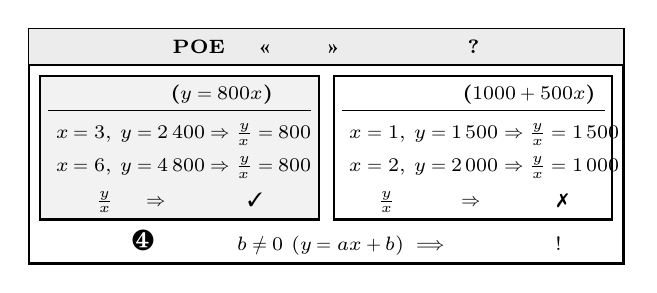
\begin{tikzpicture}[x=1cm, y=1cm, every node/.style={font=\scriptsize, text=black}]
  \draw[black, line width=0.9pt] (0,0) rectangle (7.55,2.98);
  \fill[gray!15] (0,2.52) rectangle (7.55,2.98);
  \draw[black, line width=0.6pt] (0,2.52) -- (7.55,2.52);
  \node at (3.775,2.75) {\textbf{\en{POE}៖ តើ «កើនទាំងពីរ» សុទ្ធតែជាសមាមាត្រស្របឬ?}};

  % ឆ្វេង៖ ករណី ក (សមាមាត្រស្រប)
  \draw[black, line width=0.8pt, fill=gray!10] (0.14,0.56) rectangle (3.68,2.38);
  \node at (1.91,2.14) {\textbf{ករណី ក៖ សៀវភៅ ($y=800x$)}};
  \draw[black, line width=0.45pt] (0.24,1.94) -- (3.58,1.94);
  \node[anchor=west] at (0.22,1.64) {$x=3,\; y=2\,400 \Rightarrow \frac{y}{x}=800$};
  \node[anchor=west] at (0.22,1.22) {$x=6,\; y=4\,800 \Rightarrow \frac{y}{x}=800$};
  \node at (1.91,0.78) {\textbf{$\frac{y}{x}$ ថេរ $\Rightarrow$ សមាមាត្រស្រប \ding{51}}};

  % ស្ដាំ៖ ករណី ខ (អន្ទាក់ថ្លៃដើមថេរ)
  \draw[black, line width=0.8pt] (3.87,0.56) rectangle (7.41,2.38);
  \node at (5.64,2.14) {\textbf{ករណី ខ៖ ផ្ញើឥវ៉ាន់ ($1000+500x$)}};
  \draw[black, line width=0.45pt] (3.97,1.94) -- (7.31,1.94);
  \node[anchor=west] at (3.95,1.64) {$x=1,\; y=1\,500 \Rightarrow \frac{y}{x}=1\,500$};
  \node[anchor=west] at (3.95,1.22) {$x=2,\; y=2\,000 \Rightarrow \frac{y}{x}=1\,000$};
  \node at (5.64,0.78) {\textbf{$\frac{y}{x}$ ប្រែប្រួល $\Rightarrow$ មិនសមាមាត្រ \ding{55}}};

  \node at (3.775,0.26) {\textbf{គន្លឹះ \cnum{4}៖} មានតួបូកថេរ $b\neq 0$ ($y = ax + b$) $\implies$ \textbf{មិនមែន}សមាមាត្រស្រប!};
\end{tikzpicture}}

% ៤. E4 Elaborate: ប្លង់វិភាគ ៣ ជំហាន រក x, y, a -> y = ax (បណ្ណាល័យ ទំ.២៨)
\newcommand{\figElaboratePROPThreeOneOne}{%
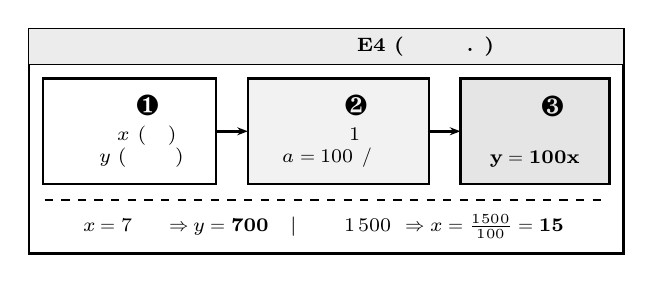
\begin{tikzpicture}[x=1cm, y=1cm, every node/.style={font=\scriptsize, text=black}]
  \draw[black, line width=0.9pt] (0,0) rectangle (7.55,2.85);
  \fill[gray!15] (0,2.40) rectangle (7.55,2.85);
  \draw[black, line width=0.6pt] (0,2.40) -- (7.55,2.40);
  \node at (3.775,2.625) {\textbf{ប្លង់វិភាគ ៣ ជំហានលើសន្លឹកកិច្ចការ \en{E4} (បណ្ណាល័យ ទំ.២៨)}};

  \draw[black, line width=0.8pt, fill=white] (0.18,0.88) rectangle (2.38,2.22);
  \node[align=center] at (1.28,1.55) {\textbf{ជំហាន \cnum{1}}\\[1pt]កំណត់ $x$ (ថ្ងៃ)\\និង $y$ (ប្រាក់ \riel)};

  \draw[black, line width=0.8pt, fill=gray!10] (2.78,0.88) rectangle (5.08,2.22);
  \node[align=center] at (3.93,1.55) {\textbf{ជំហាន \cnum{2}}\\[1pt]មេគុណក្នុង $1$ ថ្ងៃ\\$a = 100\riel/\text{ថ្ងៃ}$};

  \draw[black, line width=1.0pt, fill=gray!20] (5.48,0.88) rectangle (7.37,2.22);
  \node[align=center] at (6.425,1.55) {\textbf{ជំហាន \cnum{3}}\\[1pt]សរសេរសមីការ\\$\mathbf{y = 100x}$};

  \draw[black, line width=0.9pt, -{Stealth[length=3.8pt]}] (2.38,1.55) -- (2.78,1.55);
  \draw[black, line width=0.9pt, -{Stealth[length=3.8pt]}] (5.08,1.55) -- (5.48,1.55);

  \draw[black, line width=0.65pt, dashed] (0.20,0.68) -- (7.35,0.68);
  \node at (3.775,0.34) {ហួស $x=7$ ថ្ងៃ $\Rightarrow y = \mathbf{700\riel}$ \;\textbar{}\; ពិន័យ $1\,500\riel \Rightarrow x = \frac{1500}{100} = \mathbf{15}$ ថ្ងៃ};
\end{tikzpicture}}

% ៥. E5 Evaluate: ជម្រើសវិនិច្ឆ័យ ៤ ទម្រង់ A-D (លើកម្រាមដៃ ១-៤ + គូសរង្វង់លើសន្លឹកកិច្ចការ)
\newcommand{\figExitPROPThreeOneOne}{%
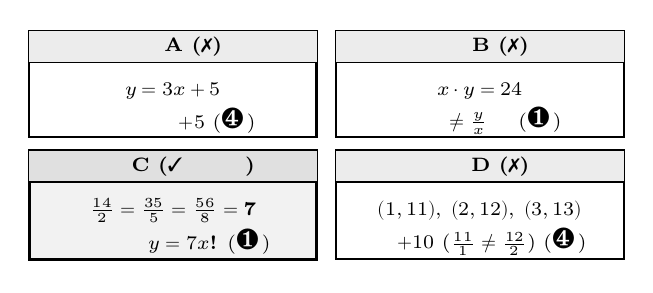
\begin{tikzpicture}[x=1cm, y=1cm, every node/.style={font=\scriptsize, text=black}]
  % A
  \draw[black, line width=0.8pt] (0,1.55) rectangle (3.65,2.90);
  \fill[gray!15] (0,2.50) rectangle (3.65,2.90);
  \draw[black, line width=0.55pt] (0,2.50) -- (3.65,2.50);
  \node at (1.825,2.70) {\textbf{ជម្រើស \en{A} (\ding{55})}};
  \node at (1.825,2.14) {$y = 3x + 5$};
  \node at (1.825,1.76) {អន្ទាក់តួបូកថេរ $+5$ (\cnum{4})};

  % B
  \draw[black, line width=0.8pt] (3.90,1.55) rectangle (7.55,2.90);
  \fill[gray!15] (3.90,2.50) rectangle (7.55,2.90);
  \draw[black, line width=0.55pt] (3.90,2.50) -- (7.55,2.50);
  \node at (5.725,2.70) {\textbf{ជម្រើស \en{B} (\ding{55})}};
  \node at (5.725,2.14) {$x\cdot y = 24$};
  \node at (5.725,1.76) {ផលគុណថេរ $\neq \frac{y}{x}$ ថេរ (\cnum{1})};

  % C (Correct)
  \draw[black, line width=1.1pt, fill=gray!10] (0,0) rectangle (3.65,1.38);
  \fill[gray!24] (0,0.98) rectangle (3.65,1.38);
  \draw[black, line width=0.6pt] (0,0.98) -- (3.65,0.98);
  \node at (1.825,1.18) {\textbf{ជម្រើស \en{C} (\ding{51} ត្រឹមត្រូវ)}};
  \node at (1.825,0.62) {$\frac{14}{2}=\frac{35}{5}=\frac{56}{8}=\mathbf{7}$};
  \node at (1.825,0.22) {\textbf{សមាមាត្រស្រប $y=7x$!} (\cnum{1})};

  % D
  \draw[black, line width=0.8pt] (3.90,0) rectangle (7.55,1.38);
  \fill[gray!15] (3.90,0.98) rectangle (7.55,1.38);
  \draw[black, line width=0.55pt] (3.90,0.98) -- (7.55,0.98);
  \node at (5.725,1.18) {\textbf{ជម្រើស \en{D} (\ding{55})}};
  \node at (5.725,0.62) {$(1,11),\; (2,12),\; (3,13)$};
  \node at (5.725,0.22) {បូក $+10$ ($\frac{11}{1}\neq\frac{12}{2}$) (\cnum{4})};
\end{tikzpicture}}

% ============================================================================
% ចាប់ផ្ដើមឯកសារ (Document Body)
% ============================================================================
\begin{document}
\fontsize{10pt}{15.2pt}\selectfont

% -------------------- ក្បាលកិច្ចតែងការ (Header) --------------------
\begin{center}
  {\muol\fontsize{11pt}{16pt}\selectfont ព្រះរាជាណាចក្រកម្ពុជា}\\[2pt]
  {\muol\fontsize{10pt}{15pt}\selectfont ជាតិ សាសនា ព្រះមហាក្សត្រ}\\[1pt]
  \khmflourish
\end{center}

\vspace{-24pt}
{\muol\fontsize{9.5pt}{12.5pt}\selectfont
មន្ទីរអប់រំ យុវជន និងកីឡា ខេត្តកំពង់ធំ\\
ការិយាល័យអប់រំ យុវជន និងកីឡា ស្រុកកំពង់ស្វាយ\\
អនុវិទ្យាល័យព្រះក្រសាំង}

\vspace{1pt}
\begin{center}
  {\muol\fontsize{10pt}{14pt}\selectfont កិច្ចតែងការបង្រៀន}
\end{center}
\vspace{0pt}

% -------------------- ព័ត៌មានទូទៅ (Metadata) --------------------
{\renewcommand{\arraystretch}{0.98}
\hspace*{3.1cm}%
\begin{tabular}{@{}l l L{11.0cm}@{}}
  - \hspace{0.35cm} មុខវិជ្ជា & : & គណិតវិទ្យា ថ្នាក់ទី៨ (ពីជគណិត) \\
  - \hspace{0.35cm} ចំណងជើងមេរៀន & : & មេរៀនទី៣៖ ទំហំសមាមាត្រនិងភាគរយ \\
  - \hspace{0.35cm} ចំណងជើងរង & : & ១. ទំហំសមាមាត្រ — ១.១. ទំហំសមាមាត្រស្រប (ទំ.២៧–២៨, ៤០–៤១) \\
  - \hspace{0.35cm} រយៈពេល & : & ១ ម៉ោងសិក្សា (៥០ នាទី) \\
  - \hspace{0.35cm} បង្រៀនដោយ & : & ហុក ប៊ុនថែន \\
  - \hspace{0.35cm} កាលបរិច្ឆេទ & : & ថ្ងៃអង្គារ ទី១៧ ខែវិច្ឆិកា ឆ្នាំ២០២៦ \\
\end{tabular}

\vspace{2pt}

% -------------------- I. វត្ថុបំណង --------------------
\textbf{I.} {\muol វត្ថុបំណង}\\[1pt]
\hspace*{0.55cm}%
\begin{tabular}{@{}l l L{14.2cm}@{}}
  \wcirc \hspace{0.25cm} វិជ្ជាសម្បទា & : & សិស្សប្រាប់និយមន័យទំហំសមាមាត្រស្រប មេគុណសមាមាត្រ $a \neq 0$ និងសរសេរទំនាក់ទំនង $\frac{y}{x} = a$ ឬ $y = ax$ ព្រមទាំងញែកដាច់ពីទំនាក់ទំនងបូកបន្ថែម $y = ax + b$ ($b\neq 0$) បានត្រឹមត្រូវតាមសៀវភៅសិក្សាគោល ។ \\
  \wcirc \hspace{0.25cm} បំណិនសម្បទា & : & សិស្សបំពេញតារាងផលធៀប (\en{Ratio Table}) គណនាមេគុណសមាមាត្រ $a$ និងបង្កើតសមីការដោះស្រាយចំណោទជាក់ស្ដែង (ប្រាក់ពិន័យបណ្ណាល័យ ចម្ងាយចរយន្តហោះ និងថ្លៃទំនិញ ទំ.២៧–២៨, ៤០–៤១) នៅលើសន្លឹកកិច្ចការបានត្រឹមត្រូវ ។ \\
  \wcirc \hspace{0.25cm} ចរិយាសម្បទា & : & សិស្សមានទម្លាប់ផ្ទៀងផ្ទាត់ផលធៀប $\frac{y}{x}$ មុនសន្និដ្ឋាន សហការពិភាក្សាជាគូលើសន្លឹកកិច្ចការយ៉ាងសកម្ម និងគោរពវិន័យពេលខ្ចីសៀវភៅបណ្ណាល័យ ឬទិញដូរប្រចាំថ្ងៃដោយស្មោះត្រង់ ។ \\
\end{tabular}

\vspace{2pt}

% -------------------- II. សម្ភារៈឧបទេស --------------------
\textbf{II.} {\muol សម្ភារៈឧបទេស}\\[1pt]
\hspace*{0.55cm}$\bullet$ \hspace{0.35cm} សៀវភៅសិក្សាគោលគណិតវិទ្យាថ្នាក់ទី៨ (ទំ.២៧–២៨, ៤០–៤១) ក្ដារខៀន ដីស/ហ្វឺត បន្ទាត់ត្រង់ និង\textbf{សន្លឹកកិច្ចការសិស្សបំពេញចន្លោះ ស-ខ្មៅ} (\en{Printable\_Materials\_PROP311} ទំព័រ ១–២ សម្រាប់សិស្ស និងទំព័រ ៣ ប្លង់ក្ដារខៀន/ចម្លើយសម្រាប់គ្រូ — គ្មានប្រើ \en{LCD})

\vspace{2pt}

% -------------------- III. វិធីសាស្រ្តបង្រៀន --------------------
\textbf{III.} {\muol វិធីសាស្រ្តបង្រៀន}\\[1pt]
\hspace*{0.45cm}%
\begin{tabular}{@{}l l L{14.85cm}@{}}
  $\bullet$ \hspace{0.25cm} គោលវិធី & : & សិស្សមជ្ឈមណ្ឌល (បង្រៀនដោយប្រើសន្លឹកកិច្ចការបំពេញចន្លោះជាគោល និងក្ដារខៀន) \\
  $\bullet$ \hspace{0.25cm} យុទ្ធវិធីបង្រៀន & : & គំរូស្ថាបនានិយម \en{5Es} រួមបញ្ចូល \textbf{តារាងផលធៀប (\en{Ratio Table})}, \textbf{\en{POE} ករណីប្រៀបធៀបផ្ទុយគ្នា (\en{Contrasting Cases})} និង\textbf{លំហាត់គំរូបន្ថយជំនួយ (\en{Faded Worked Examples})} \\
\end{tabular}
}

\vspace{2pt}

% -------------------- IV. ដំណើរការបង្រៀន --------------------
\textbf{IV.} {\muol ដំណើរការបង្រៀន}

\vspace{1pt}

% ============================================================================
% តារាងដំណើរការបង្រៀន (Granular 2-5 Line Sub-Rows, Dedicated TikZ Rows, 50 min)
% ============================================================================
\renewcommand{\arraystretch}{1.15}
\begin{longtable}{|L{5.50cm}|L{7.90cm}|L{4.80cm}|}
\hline
\rowcolor{headgray}
\multicolumn{1}{|c|}{\muol សកម្មភាពគ្រូ} &
\multicolumn{1}{c|}{\muol ខ្លឹមសារមេរៀន} &
\multicolumn{1}{c|}{\muol សកម្មភាពសិស្ស} \\
\hline
\endfirsthead

\hline
\endhead

\hline
\endfoot

\hline
\endlastfoot

% ==================== ជំហានទី១ (2min) ====================
\stepheader{ជំហានទី១ \enbf{(}រដ្ឋបាលថ្នាក់\enbf{)}}
$\bullet$ ពិនិត្យអវត្តមាន អនាម័យ និងសណ្ដាប់ធ្នាប់ថ្នាក់រៀន
&
$\bullet$ ពិនិត្យវត្តមានសិស្ស អនាម័យ និងសណ្ដាប់ធ្នាប់ក្នុងថ្នាក់
&
$\circ$ ប្រធានថ្នាក់រាយការណ៍វត្តមានសិស្ស \\[3pt]

$\bullet$ រៀបចំសិស្សអង្គុយជាគូ (២ នាក់ក្នុង ១ តុ) \par
$\bullet$ ចែក\textbf{សន្លឹកកិច្ចការសិស្ស (ទំព័រ ១–២)} ម្នាក់ ១ សន្លឹក ដោយឱ្យសរសេរឈ្មោះទុកជាមុន
&
$\bullet$ របៀបធ្វើការ៖ បំពេញសន្លឹកកិច្ចការតាមជំហាន \en{E1}--\en{E5} និងផ្ទៀងផ្ទាត់ជាមួយដៃគូតុជាប់គ្នា
&
$\circ$ ទទួលសន្លឹកកិច្ចការ សរសេរឈ្មោះ និងត្រៀមប៊ិក/ខ្មៅដៃ \\
\hline

% ==================== ជំហានទី២ (9min: <=3 + 3 + E1 3) ====================
\stepheader{ជំហានទី២ \enbf{(}កិច្ចការផ្ទះ \enbf{+} ទំនាក់ទំនងមេរៀនថ្មី\enbf{)}}
% --- ២.១ កំណែកិច្ចការផ្ទះ (<=3min) ---
\ditem \textbf{កំណែកិច្ចការផ្ទះ ($\le 3\unit{min}$)} \par
$\bullet$ ហៅសិស្ស ២ នាក់ឡើងកែលំហាត់បញ្ចប់មេរៀនទី២ (ការបម្លែងទសភាគ និងស្វ័យគុណនៃ $10$) លើក្ដារខៀនយ៉ាងរហ័ស
&
{\centering\redsub{កំណែកិច្ចការផ្ទះមេរៀនមុន (មេរៀនទី២ ទំ.២៦)}\par} \par
$\bullet$ \textbf{ក.} $\dfrac{2}{10} = 2\times 10^{-1} = 0.2$ \quad \textbar{} \quad \textbf{ខ.} $3.5\times 10^2 = 350$ \par
\timenote{(ភ្ជាប់មកការសម្រួលប្រភាគជាចំនួនទសភាគ $0.2$ សម្រាប់មេរៀនថ្មី)}
&
$\circ$ ផ្ទៀងផ្ទាត់ចម្លើយលើក្ដារខៀន និងកែតម្រូវក្នុងសៀវភៅកិច្ចការ \\[3pt]

% --- ២.២ រំលឹកមេរៀនចាស់ (3min) ---
\ditem \textbf{រំលឹកមេរៀនទាក់ទង (3min)} \par
$\bullet$ សរសេរប្រភាគ ៣ លើក្ដារខៀន រួចសួរ៖ \par
\hspace*{0.3em}– «ចូរសម្រួលប្រភាគ $\frac{10}{50},\; \frac{20}{100},\; \frac{30}{150}$ ជាទសភាគ!» \par
\hspace*{0.3em}– «បើ $\frac{y}{x} = a$ ($x\neq 0$) តើទាញរក $y$ បានដូចម្ដេច?»
&
{\centering\redsub{រំលឹកមេរៀនទាក់ទងមេរៀនថ្មី}\par} \par
$\bullet$ \textbf{ផលធៀបស្មើគ្នា៖} $\dfrac{10}{50} = \dfrac{20}{100} = \dfrac{30}{150} = \dfrac{1}{5} = 0.2$ \par
$\bullet$ \textbf{ទំនាក់ទំនងចែកនិងគុណ៖} បើ $\dfrac{y}{x} = a \implies y = a\cdot x$ ($x\neq 0$)
&
$\circ$ គិតរហ័ស និងឆ្លើយព្រមគ្នា៖ «ស្មើ $0.2$ ដូចគ្នា!» និង «$y = ax$» \\[3pt]

% --- ២.៣ E1 Engage (3min) ---
\fiveE{E1 - Engage (3min)} \timenote{(កុំទាន់ផ្ដល់ចម្លើយ)} \par
\ditem \textbf{បេសកកម្មលើសន្លឹកកិច្ចការផ្នែក \en{E1}៖} \par
$\bullet$ ឱ្យសិស្សមើល \textbf{ប្រអប់ \en{E1}} លើសន្លឹកកិច្ចការ (ទំព័រ ១) អំពីស្ថានភាព ២ នៅផ្សារព្រះក្រសាំង និងអាយុបងប្អូន
&
{\centering\redsub{បេសកកម្ម E1៖ «កើនដូចគ្នា» តែហេតុអ្វីគុណមិនត្រូវដូចគ្នា?}\par} \par
$\bullet$ \textbf{ក. សៀវភៅសរសេរ៖} $2$ ក្បាលថ្លៃ $1\,600\riel \implies 6$ ក្បាលថ្លៃ $4\,800\riel$ \par
$\bullet$ \textbf{ខ. អាយុបងប្អូន៖} ដារ៉ា $2$ ឆ្នាំ បងសុខា $6$ ឆ្នាំ។ ពេលដារ៉ាអាយុ $6$ ឆ្នាំ តើសុខាអាយុ $18$ ឆ្នាំ ឬ $10$ ឆ្នាំ?
&
$\circ$ អានប្រអប់ \en{E1} លើសន្លឹកកិច្ចការ និងពិភាក្សាជាគូរយៈពេល ១ នាទី \\[3pt]

&
\cfig{\figEngagePROPThreeOneOne}
& \\[3pt]

\hspace*{0.3em}– \textbf{សំណួរំញោច៖} «ស្ថានភាពទាំងពីរសុទ្ធតែកើនឡើងដូចគ្នា! ហេតុអ្វីថ្លៃសៀវភៅគុណនឹង $3$ ត្រូវ ឯអាយុបងសុខាគុណនឹង $3$ បែរជាខុស?»
&
$\bullet$ \textbf{ចម្ងល់គន្លឹះ៖} តើលក្ខខណ្ឌពិតប្រាកដអ្វីដែលធ្វើឱ្យទំហំពីរហៅថា \textbf{«ទំហំសមាមាត្រស្រប»}?
&
$\circ$ គូសរង្វង់ការទស្សន៍ទាយក្នុងប្រអប់ \en{E1} លើសន្លឹកកិច្ចការ (រង់ចាំផ្ទៀងនៅ \en{E5}) \\
\hline

% ==================== ជំហានទី៣ (17min: E2 11m + E3 6m) ====================
\stepheader{ជំហានទី៣ \enbf{(}ខ្លឹមសារមេរៀនថ្មី\enbf{)}}
% --- ៣.១ ចំណងជើង & E2 Act 1 (5min) ---
\fiveE{E2 - Explore (11min)} \par
$\bullet$ សរសេរចំណងជើងមេរៀនទី៣ និងចំណងជើងរងលើក្ដារខៀន
&
មេរៀនទី៣ \hspace{0.15cm} {\muol ទំហំសមាមាត្រនិងភាគរយ} \par
\textbf{១. ទំហំសមាមាត្រ} \quad \textbar{} \quad \textbf{១.១. ទំហំសមាមាត្រស្រប}
&
$\circ$ កត់ចំណងជើងមេរៀនចូលសៀវភៅសរសេរ \\[3pt]

\ditem \textbf{សកម្មភាព ១៖ តារាងផលធៀបជញ្ជីងដៃ (5min, សន្លឹកកិច្ចការ \en{E2-A})} \par
$\bullet$ ណែនាំ \textbf{ឧទាហរណ៍ជញ្ជីងដៃថ្លឹងម៉ាស (ទំ.២៧)} និងឱ្យសិស្សបំពេញតារាងជួរទី៣ ($\frac{y}{x}$) ព្រមទាំងប្រអប់ទំនេរចុងក្រោយ ($x=300\unit{g}$)
&
{\centering\textbf{សកម្មភាព ១៖ ឧទាហរណ៍ជញ្ជីងដៃថ្លឹងម៉ាស (សៀវភៅគោល ទំ.២៧)}\par} \par
$\bullet$ ម៉ាស $x\unit{(g)}$៖ $50,\; 100,\; 150,\; 250,\; [300]$ \par
$\bullet$ ប្រវែងរ៉ឺស័រលូត $y\unit{(mm)}$៖ $10,\; 20,\; 30,\; 50,\; [60]$ \par
$\bullet$ ពិនិត្យផលធៀប៖ $\dfrac{y}{x} = \dfrac{10}{50} = \dfrac{20}{100} = \dfrac{30}{150} = \dfrac{50}{250} = \mathbf{0.2}$
&
$\circ$ គណនាផលធៀប $\frac{y}{x}$ គ្រប់ជួរឈរ និងបំពេញតម្លៃ $[300\unit{g} \to 60\unit{mm}]$ លើសន្លឹកកិច្ចការ \\[3pt]

$\bullet$ ឱ្យសិស្សគូសព្រួញពង្រីកតាមដេក ($\times 2, \times 3, \times 5$) និងព្រួញតាមឈរ ($\times 0.2$) លើតារាង \par
\hspace*{0.3em}– \textbf{សំណួរ៖} «ពេលម៉ាស $x$ កើន $2$ ដង ឬ $5$ ដង តើប្រវែងលូត $y$ ប្រែប្រួលដូចម្ដេច? ហើយ $\frac{y}{x}$ ស្មើប៉ុន្មានជានិច្ច?»
&
$\bullet$ \textbf{សង្កេតតាមដេក៖} កាលណាម៉ាស $x$ កាន់តែធំប៉ុន្មានដង ប្រវែងរ៉ឺស័រលូត $y$ ក៏កាន់តែវែងទៅតាម\textbf{ចំនួនដង}នៃម៉ាសដែរ ។ \par
$\bullet$ \textbf{សង្កេតតាមឈរ៖} $\dfrac{y}{x} = 0.2$ ឬ $y = 0.2x$ \par
$\implies$ គេថា $x$ និង $y$ ជា\textbf{ទំហំសមាមាត្រស្រប} និង $0.2$ ជា\textbf{មេគុណសមាមាត្រ} ។
&
$\circ$ គូសព្រួញលើតារាងសន្លឹកកិច្ចការ និងឆ្លើយ៖ «$y$ កើនតាមចំនួនដងស្មើគ្នា ហើយ $\frac{y}{x}=0.2$ ថេរ!» \\[3pt]

&
\cfig{\figExploreSpringPROPThreeOneOne}
& \\[3pt]

% --- ៣.២ E2 Act 2 POE Contrasting Cases (6min) ---
\ditem \textbf{សកម្មភាព ២៖ \en{POE} ករណីប្រៀបធៀបបំបែកអន្ទាក់បូក (6min, សន្លឹកកិច្ចការ \en{E2-B})} \par
$\bullet$ ឱ្យសិស្ស \textbf{ទស្សន៍ទាយ (\en{P})} មុនគណនាលើតារាងទាំងពីរ៖ \par
\hspace*{0.3em}– \textbf{ករណី ក៖} សៀវភៅ $3$ ក្បាល $2\,400\riel$, $6$ ក្បាល $4\,800\riel$, $12$ ក្បាល $9\,600\riel$ \par
\hspace*{0.3em}– \textbf{ករណី ខ៖} ផ្ញើឥវ៉ាន់មានថ្លៃសេវាដើម $1\,000\riel$ បូក $500\riel/\text{kg}$ ($1\unit{kg}\to 1\,500\riel$, $2\unit{kg}\to 2\,000\riel$, $4\unit{kg}\to 3\,000\riel$)
&
{\centering\textbf{\en{POE}៖ ករណីប្រៀបធៀបផ្ទុយគ្នា (\en{Contrasting Cases})}\par} \par
$\bullet$ \textbf{ទស្សន៍ទាយ (\en{P})៖} សិស្សខ្លះស្មានថា ករណី ខ ក៏សមាមាត្រស្របដែរ ព្រោះទម្ងន់កើន ថ្លៃផ្ញើក៏កើន ។ \par
$\bullet$ \textbf{សង្កេត (\en{O})៖} គណនាផលធៀប $\dfrac{y}{x}$ លើសន្លឹកកិច្ចការ៖ \par
\hspace*{0.4em}– ករណី ក៖ $\dfrac{2\,400}{3} = \dfrac{4\,800}{6} = \dfrac{9\,600}{12} = \mathbf{800}$ (ថេរ \ding{51}) \par
\hspace*{0.4em}– ករណី ខ៖ $\dfrac{1\,500}{1} = 1\,500 \neq \dfrac{2\,000}{2} = 1\,000 \neq \dfrac{3\,000}{4} = 750$ (\ding{55})
&
$\circ$ ទស្សន៍ទាយ រួចគណនាផលចែក $\frac{y}{x}$ ទាំងពីរតារាងនៅលើសន្លឹកកិច្ចការ និងភ្ញាក់ផ្អើលពេលឃើញករណី ខ មិនស្មើគ្នា \\[3pt]

$\bullet$ ឱ្យគូសិស្ស \textbf{ពន្យល់ (\en{E})} ហេតុផលដែលករណី ខ មិនមែនសមាមាត្រស្រប
&
$\bullet$ \textbf{ពន្យល់ (\en{E})៖} គ្រាន់តែ «$x$ កើន ហើយ $y$ កើន» \textbf{មិនទាន់គ្រប់គ្រាន់ទេ}! លុះត្រាតែផលធៀប $\dfrac{y}{x} = a$ ថេរគ្រប់គូតម្លៃ (គ្មានតួបូកថេរ $b\neq 0$) ។
&
$\circ$ សរសេរសេចក្ដីសន្និដ្ឋាន \en{POE} ក្នុងប្រអប់សន្លឹកកិច្ចការ \\[3pt]

&
\cfig{\figPOEContrastPROPThreeOneOne}
& \\[3pt]

% --- ៣.៣ E3 Explain (6min) ---
\fiveE{E3 - Explain (6min)} \par
\ditem \textbf{បង្គុំប្រអប់ «ជាទូទៅ» (ទំ.២៧)} \par
$\bullet$ ហៅតំណាងគូឡើងបំពេញប្រអប់ «ជាទូទៅ» លើក្ដារខៀន និងបញ្ជាក់លក្ខខណ្ឌ $a \neq 0$
&
\textbf{ជាទូទៅ (ទំ.២៧)៖} $y$ និង $x$ ជាទំហំសមាមាត្រស្រប និង $a \neq 0$ ជាមេគុណសមាមាត្រ គេបាន៖ \graybox{$\dfrac{y}{x} = a \quad \text{ឬ} \quad y = ax$} ។
&
$\circ$ បំពេញប្រអប់ «ជាទូទៅ» លើសន្លឹកកិច្ចការផ្នែក \en{E3} និងកត់ចូលសៀវភៅ \\[3pt]

$\bullet$ សង្ខេបតារាង \textbf{សម្មតិកម្ម--សន្និដ្ឋាន--វិបាក} និងភ្ជាប់\textbf{ធនាគារហេតុផល \cnum{1}--\cnum{4}} នៅលើសន្លឹកកិច្ចការ
&
{\fontsize{8.8pt}{12.6pt}\selectfont\setlength{\tabcolsep}{2.5pt}\renewcommand{\arraystretch}{1.14}%
\centering
\begin{tabular}{|L{2.25cm}|L{2.45cm}|L{2.65cm}|}
  \hline
  \cellcolor{headgray}\textbf{សម្មតិកម្ម} & \cellcolor{headgray}\textbf{សន្និដ្ឋាន} & \cellcolor{headgray}\textbf{វិបាក / អន្ទាក់សំខាន់} \\
  \hline
  $y$ សមាមាត្រស្របនឹង $x$ មេគុណ $a\neq 0$ & $\dfrac{y}{x} = a \iff y = ax$ & $x = \dfrac{y}{a}$; បើ $x$ កើន $k$ ដង $\Rightarrow y$ កើន $k$ ដង \\
  \hline
  ទំនាក់ទំនងមានតួបូក $y = ax + b$ ($b\neq 0$) & $\dfrac{y}{x} = a + \dfrac{b}{x}$ (ប្រែប្រួល) & \textbf{មិនមែន}ទំហំសមាមាត្រស្របឡើយ! \\[2pt]
  \hline
\end{tabular}\par}
&
$\circ$ ផ្ទៀងតារាងសង្ខេប និងគូសបន្ទាត់ក្រោមពាក្យគន្លឹះ \\[3pt]

$\bullet$ ណែនាំលេខកូដហេតុផល \cnum{1}--\cnum{4} សម្រាប់សម្គាល់ពេលដោះស្រាយលំហាត់
&
\textbf{ធនាគារហេតុផល (\en{Warrant Bank} លើសន្លឹកកិច្ចការ)៖} \par
\cnum{1} តេស្តផលធៀបថេរ៖ $\dfrac{y}{x} = a$ (មេគុណសមាមាត្រ = តម្លៃក្នុង $1$ ឯកតា) \par
\cnum{2} រូបមន្តសមាមាត្រស្រប៖ $y = ax$ និងទាញរក $x = \dfrac{y}{a}$ \par
\cnum{3} ពង្រីកតាមចំនួនដង៖ $x$ គុណនឹង $k \implies y$ គុណនឹង $k$ ដូចគ្នា \par
\cnum{4} អន្ទាក់ការគិតបែបបូក៖ $y = ax + b$ ($b\neq 0$) មិនមែនសមាមាត្រស្របទេ
&
$\circ$ ផ្ទៀងលេខកូដ \cnum{1}--\cnum{4} លើសន្លឹកកិច្ចការសម្រាប់ប្រើក្នុង \en{E4} និង \en{E5} \\
\hline

% ==================== ជំហានទី៤ (20min: E4 10m + E5 10m) ====================
\stepheader{ជំហានទី៤ \enbf{(}ពង្រីកចំណេះដឹង\enbf{)}}
% --- ៤.១ E4 Elaborate (10min) ---
\fiveE{E4 - Elaborate (10min)} \par
\ditem \textbf{លំហាត់គំរូបន្ថយជំនួយ ៣ ជំហាន (សន្លឹកកិច្ចការ \en{E4})} \par
$\bullet$ ដឹកនាំ \textbf{លំហាត់គំរូទី ១ (បណ្ណាល័យ ទំ.២៨)}៖ គូសរង្វង់តម្លៃក្នុង $1$ ថ្ងៃ ($100\riel$)
&
{\muol លំហាត់គំរូទី ១} \textbf{(សៀវភៅគោល ទំ.២៨ — ប្រាក់ពិន័យបណ្ណាល័យ)៖} \par
សងសៀវភៅហួសកំណត់ $1$ ថ្ងៃ ត្រូវពិន័យប្រាក់ $100\riel$ ។ \par
$\bullet$ \textbf{ជំហានទី ១៖} តាង $x$ ជាចំនួនថ្ងៃហួសកំណត់ និង $y$ ជាប្រាក់ពិន័យ $(\riel)$
&
$\circ$ គូសរង្វង់តម្លៃក្នុង $1$ ថ្ងៃ និងកំណត់អថេរ $x, y$ \\[3pt]

$\bullet$ ឱ្យសិស្សបំពេញជំហានទី ២ និងទី ៣ លើសន្លឹកកិច្ចការ រួចគណនាករណី $7$ ថ្ងៃ និង $1\,500\riel$
&
$\bullet$ \textbf{ជំហានទី ២៖} ប្រាក់ពិន័យកើនតាមចំនួនដងនៃថ្ងៃ $\implies a = 100\riel/\text{ថ្ងៃ}$ (\cnum{1}) \par
$\bullet$ \textbf{ជំហានទី ៣៖} សមីការទំនាក់ទំនងគឺ \graybox{$y = 100x$} (\cnum{2})
&
$\circ$ បំពេញ $a=100$ និងសមីការ $y=100x$ លើសន្លឹកកិច្ចការ \\[3pt]

&
\cfig{\figElaboratePROPThreeOneOne}
& \\[3pt]

$\bullet$ ដឹកនាំ \textbf{លំហាត់គំរូទី ២ (ទំ.៤០ \#6 ក — សៀវភៅសរសេរ)} តាមរបៀបទី ១ (តម្លៃឯកតា $a$)
&
{\muol លំហាត់គំរូទី ២} \textbf{(ទំ.៤០ \#6 ក — ថ្លៃសៀវភៅសរសេរ)៖} \par
សៀវភៅសរសេរ $6$ ក្បាលថ្លៃ $4\,800\riel$ ។ រកថ្លៃសៀវភៅសរសេរ $12$ ក្បាល៖ \par
$\bullet$ \textbf{របៀបទី ១ (\cnum{1}--\cnum{2})៖} $a = \dfrac{4\,800}{6} = 800\riel/\text{ក្បាល} \implies y = 800\times 12 = \mathbf{9\,600\riel}$
&
$\circ$ គណនាថ្លៃ $1$ ក្បាល ($800\riel$) រួចគុណនឹង $12$ \\[3pt]

$\bullet$ បង្ហាញប្រៀបធៀបជាមួយ\textbf{របៀបទី ២ (តាមចំនួនដង $k$)}
&
$\bullet$ \textbf{របៀបទី ២ (តាមចំនួនដង, \cnum{3})៖} $12$ ក្បាល $= 2\times 6$ ក្បាល $\implies y = 2\times 4\,800 = \mathbf{9\,600\riel}$
&
$\circ$ បំពេញរបៀបទី ២ និងប្រៀបធៀបភាពរហ័ស \\[3pt]

$\bullet$ សួរសំណួរឆ្លុះបញ្ចាំង \textbf{\en{EIA Looking-Back} (30 វិនាទី)}
&
\textbf{\en{EIA Looking-Back}៖} «ហេតុអ្វីមុនគណនា $a = \frac{y}{x}$ យើងត្រូវបញ្ជាក់ខ្នាតរបស់ $x$ និង $y$ ឱ្យច្បាស់ជានិច្ច?» ($\to$ ដើម្បីដឹងអត្ថន័យមេគុណ $a$ ក្នុង $1$ ឯកតា ដូចជា $\riel/\text{ក្បាល}$ ឬ $\unit{km/h}$)
&
$\circ$ ឆ្លើយបញ្ជាក់អត្ថន័យខ្នាតនៃមេគុណសមាមាត្រ $a$ \\[3pt]

% --- ៤.២ E5 Evaluate (10min) ---
\fiveE{E5 - Evaluate (10min)} \par
\ditem \textbf{ប្រតិបត្តិជាគូតាមវិន័យ \en{Pause-Check} (6min, សន្លឹកកិច្ចការ \en{E5})} \par
$\bullet$ ឱ្យសិស្សធ្វើ \textbf{ប្រតិបត្តិទី ១ (យន្តហោះ ទំ.២៨)}
&
{\muol លំហាត់ប្រតិបត្តិ} \textbf{(សៀវភៅគោល ទំ.២៨ និង ទំ.៤១ \#6 ខ)៖} \par
$\bullet$ \textbf{១) យន្តហោះ (ទំ.២៨)៖} ល្បឿនថេរ $a = 800\unit{km/h}$, រយៈពេល $t = 8\unit{h}$ \par
\hspace*{0.4em}សមីការចម្ងាយចរ៖ $d = 800t \implies d = 800\times 8 = \graybox{$6\,400\unit{km}$}$ (\cnum{2})
&
$\circ$ សរសេរសមីការ $d=800t$ និងគណនា $6\,400\unit{km}$ \\[3pt]

$\bullet$ បន្ត \textbf{ប្រតិបត្តិទី ២ (ថ្លៃតែ ទំ.៤១ \#6 ខ)} និងប្ដូរសន្លឹកគ្នាផ្ទៀងជាមួយដៃគូ
&
$\bullet$ \textbf{២) ថ្លៃតែ (ទំ.៤១ \#6 ខ)៖} តែ $3\unit{kg}$ ថ្លៃ $45\,000\riel \implies$ រកថ្លៃតែ $10\unit{kg}$៖ \par
\hspace*{0.4em}$a = \dfrac{45\,000}{3} = 15\,000\riel/\text{kg} \implies y = 15\,000\times 10 = \graybox{$150\,000\riel$}$ (\cnum{1}, \cnum{2})
&
$\circ$ គណនាថ្លៃតែ $150\,000\riel$ និងប្ដូរសន្លឹកផ្ទៀងផ្ទាត់ជាមួយដៃគូ \\[3pt]

$\bullet$ ឱ្យសិស្សវិលទៅ \textbf{បិទបញ្ចប់បេសកកម្ម \en{E1}} នៅដើមម៉ោង
&
$\bullet$ \textbf{បិទបេសកកម្ម \en{E1}៖} ថ្លៃសៀវភៅមាន $\frac{y}{x} = 800\riel/\text{ក្បាល}$ ថេរ (\ding{51}); ចំណែកអាយុបងសុខាគឺ $y = x + 4$ (ពេលដារ៉ា $6$ ឆ្នាំ សុខាអាយុ $10$ ឆ្នាំ មិនមែន $18$ ឆ្នាំទេ ព្រោះ $\frac{6}{2}=3 \neq \frac{10}{6}$, \cnum{4}) ។
&
$\circ$ ផ្ទៀងការទស្សន៍ទាយដើមម៉ោង និងបំពេញចម្លើយបិទ \en{E1} \\[3pt]

\ditem \textbf{វាយតម្លៃរហ័ស ៤ ជម្រើស \en{A--D} និងសំបុត្រចេញ (4min)} \par
$\bullet$ ឱ្យសិស្សមើលប្រអប់ \en{A--D} លើសន្លឹកកិច្ចការ រួចលើកម្រាមដៃ (១=\en{A}, ២=\en{B}, ៣=\en{C}, ៤=\en{D}) ព្រមគ្នា (មិនប្រើក្ដារឆ្នួន មិនប្រើ \en{LCD})
&
{\centering\textbf{សំណួរវិនិច្ឆ័យ \en{A--D}៖ តើទម្រង់ណាជាទំហំសមាមាត្រស្រប?}\par}
&
$\circ$ គូសរង្វង់ជម្រើសលើសន្លឹកកិច្ចការ និងលើកម្រាមដៃបង្ហាញគ្រូ \\[3pt]

&
\cfig{\figExitPROPThreeOneOne}
& \\[3pt]

$\bullet$ បញ្ជាក់ចម្លើយត្រូវ (\textbf{ជម្រើស \en{C}}) និងឱ្យសិស្សបំពេញ \textbf{សំបុត្រចេញ ៦០ វិនាទី} នៅបាតសន្លឹកកិច្ចការទំព័រ ២
&
$\bullet$ \textbf{សំបុត្រចេញ (\en{Exit Ticket})៖} (១) បើ $y$ សមាមាត្រស្របនឹង $x$ ហើយ $x=4 \to y=28$ នោះមេគុណ $a = \mathbf{7}$ និងសមីការ $y = \mathbf{7x}$ ។ (២) តើ $y = 5x - 2$ ជាសមាមាត្រស្របឬទេ? (\textbf{ទេ} ព្រោះមានតួ $-2 \neq 0$, \cnum{4}) ។
&
$\circ$ បំពេញសំបុត្រចេញ ៦០ វិនាទីលើសន្លឹកកិច្ចការយ៉ាងរហ័ស \\
\hline

% ==================== ជំហានទី៥ (<=2min) ====================
\stepheader{ជំហានទី៥ \enbf{(}កិច្ចការផ្ទះ \enbf{+} បណ្ដាំផ្ញើ\enbf{)}}
\timenote{ចំណាយពេលឱ្យតិចបំផុតកុំឱ្យលើស 2min} \par
$\bullet$ ចង្អុលប្រអប់\textbf{កិច្ចការផ្ទះ}នៅផ្នែកខាងក្រោមសន្លឹកកិច្ចការទំព័រ ២ (សៀវភៅគោល ទំ.៤១ លេខ ៦ គ និង លេខ ១០)
&
{\centering{\muol កិច្ចការផ្ទះ} \textbf{(សៀវភៅសិក្សាគោល ទំ.៤១ លេខ ៦ គ និង លេខ ១០)}\par} \par
$\bullet$ \textbf{១) លំហាត់ ៦ គ (ទំ.៤១)៖} រកថ្លៃស្ករស $x\unit{kg}$ បើស្ករស $y\unit{kg}$ ថ្លៃ $z$ រៀល ។ \par
\hspace*{0.4em}\textit{(តម្រុយ៖ រកថ្លៃស្ករស $1\unit{kg}$ គឺ $a = \frac{z}{y}$ រៀល រួចគុណនឹង $x$ បាន $\frac{xz}{y}$ រៀល)}
&
$\circ$ គូសចំណាំកិច្ចការផ្ទះនៅលើសន្លឹកកិច្ចការ និងក្នុងសៀវភៅគោលទំ.៤១ \\[3pt]

$\bullet$ ណែនាំតម្រុយលំហាត់លេខ ១០ និងផ្ដាំផ្ញើអានមុន \textbf{១.២. លក្ខណៈនៃសមាមាត្រស្រប (ទំ.២៨–៣០)}
&
$\bullet$ \textbf{២) លំហាត់ ១០ (ទំ.៤១)៖} ប្រេងសាំង $1\unit{L}$ ថ្លៃ $3\,750\riel$ ចាក់ពេញធុងអស់ $112\,500\riel$ ។ បើប្រេងសាំងឡើងថ្លៃបន្ថែម $210\riel/\text{L}$ ចូរគណនាថ្លៃចាក់ពេញធុងឥឡូវនេះ ($= 118\,800\riel$) ។ \par
$\bullet$ \textbf{មេរៀនបន្ទាប់៖} អានមុន \textbf{លក្ខណៈនៃសមាមាត្រស្រប (ទំ.២៨–៣០)} ។
&
$\circ$ កត់ត្រាបណ្ដាំផ្ញើ ថែរក្សាសន្លឹកកិច្ចការក្នុងសៀវភៅ និងជម្រាបលាគ្រូ \\
\end{longtable}

% -------------------- កាលបរិច្ឆេទ និងហត្ថលេខា (Date & Signature) --------------------
\vspace{8pt}
\hfill
\begin{minipage}{10.5cm}
  {\centering
    ថ្ងៃអង្គារ ៨កើត ខែកត្តិក ឆ្នាំមមី អដ្ឋស័ក ពុទ្ធសករាជ ២៥៧០\\[2pt]
    កំពង់ស្វាយ, ថ្ងៃទី១៧ ខែវិច្ឆិកា ឆ្នាំ២០២៦\\[3pt]
    {\muol គ្រូបង្រៀន}\par}
  \vspace{30pt}
  \hfill{\muol ហុក ប៊ុនថែន}\hspace*{1.4cm}
\end{minipage}

\end{document}
